\documentclass[../main.tex]{subfiles}
\begin{document}
\chapter{2021-2022学年微积分（一）（下）期中考试}

\section{基本计算题(每小题 6 分，共 60 分)}
\begin{enumerate}
    \item 求微分方程$y''+9y=x\cos 3x$对应齐次方程的通解，并写出非齐次特解的待定特解形式.
          \vspace{10em}

    \item 设二阶线性微分方程$y''+a(x)y'+b(x)y=f(x)$有三个特解$y_{1}=x$，$y_{2}=x+
              2\mathrm{e}^{x}$，$y_{3}=x+(2+3x)\mathrm{e}^{x}$，求其通解.
          \vspace{11em}

    \item 已知两直线$L_{1}:
              \begin{cases}
                  x-3y+z=0, \\
                  2x-4y+z=-1
              \end{cases}$和$L_{2}:x=\frac{y+1}{3}=\frac{z-2}{4}$，求$L_{1}$与$L_{2}$之间的距离$d$.
          \vspace{11em}

    \item 设由方程$F(x-y,y-z,z-x)=0$可以确定隐函数$z=z(x,y)$，$F$具有连续的偏导数，且$F
              '_{2}-F'_{3}\neq0$，求$\mathrm{d}z$.
          \vspace{13em}

    \item 求曲线$L:
              \begin{cases}
                  x^{2}+y^{2}+z^{2}=4, \\
                  (x-1)^{2}+y^{2}=1
              \end{cases}$在点$P\left(1,1,\sqrt{2}\right)$处的法平面方程.
          \vspace{12em}

    \item 求椭圆曲线$\begin{cases}
                  z=x^{2}+y^{2}, \\
                  x+y+z=4
              \end{cases}$上距离原点最近的点.
          \vspace{12em}

    \item 计算$I=\iint\limits_{D}\left(x^{2}y^{2}+x\sin\left(x^{2}+y^{2}\right)\right
              )\,\mathrm{d}x\,\mathrm{d}y$，其中$D=\{(x,y)||x|+|y|\leq 1\}$.
          \vspace{12em}

    \item 设平面区域$D$由直线$y=x$，圆弧$y=1+\sqrt{1-x^{2}}$及$y$轴所围成，计算$I
              =\iint\limits_{D}xy\,\mathrm{d}\sigma$.
          \vspace{11em}

    \item 求二次积分$I=\int_{0}^{1}\,\mathrm{d}x\int_{x}^{1}\mathrm{e}^{-y^{2}}\,\mathrm{d}
              y$.
          \vspace{11em}

    \item 求$I=\iiint\limits_{\Omega}\frac{1}{\sqrt{x^{2}+y^{2}+z^{2}}}\,\mathrm{d}
              v$，其中$\Omega$是由曲面$z=\sqrt{x^{2}+y^{2}}$与$z=1$所围成的区域.
          \vspace{11em}
\end{enumerate}

\section{综合题(每小题 8 分，共 40 分)}
\begin{enumerate}
    \setcounter{enumi}{10}
    \item 设$z$具有二阶连续偏导数，已知变换$\begin{cases}
                  u=x-2\sqrt{y}, \\
                  v=x+2\sqrt{y}
              \end{cases}$将方程$\frac{\partial^{2} z}{\partial x^{2}}-y\frac{\partial^{2}
                  z}{\partial y^{2}}-\frac{1}{2}\frac{\partial z}{\partial y}=0$化为以$u,v$为自变量的方程，求新方程形式.
          \vspace{10em}

    \item 讨论二元函数$f(x,y)=
              \begin{cases}
                  \frac{x^2y^2}{\left(x^{2}+y^{2}\right)^{\frac{3}{2}}}, & x^{2}+y^{2}\neq 0, \\
                  0,                                                     & x^{2}+y^{2}=0
              \end{cases}$在原点$(0,0)$处的连续性、偏导数存在性及可微性.
          \vspace{11em}

    \item 求常数$a,b,c$的值，使得函数$f(x,y,z)=axy^{2}+byz+cx^{3}z^{2}$在点$M
              (1,2,-1)$处的所有方向导数中，沿$x$轴正向的方向导数最大，且该最大值为$64$.
          \vspace{11em}

    \item 求$I=\iiint\limits_{\Omega}z\,\mathrm{d}v$，其中$\Omega$是由平面曲线$\begin{cases}
                  y^{2}=2z, \\
                  x=0
              \end{cases}$绕$z$轴旋转一周所得的旋转曲面与平面$z=1$，$z=2$所围成的区域.
          \vspace{11em}

    \item 已知曲面$x^{2}+y^{2}+z=4$将球体$x^{2}+y^{2}+z^{2}\leq 4z$分为两部分，求这两部分的体积比.
          \vspace{11em}
\end{enumerate}

\chapter{2021-2022学年微积分（一）（下）期中考试参考答案}
\section{基本计算题(每小题 6 分，共 60 分)}
\begin{enumerate}
    \item \textbf{Solution}. 方程对应的齐次方程为$y''+9y=0$，其特征方程为$r^{2}+9
              =0$，解得$r=\pm 3\mathrm{i}$，

          所以齐次方程的通解为$C_{1}\cos 3x + C_{2}\sin 3x$.

          对于$y=x\cos 3x$，$\lambda = 3i$是特征方程的单根，

          所以非齐次特解的待定特解形式为$y^{*}=x\left[(Ax+B)\cos 3x + (Cx+D)\sin 3x\right
              ]$，

          其中$A,B,C,D$为待定常数.

    \item \textbf{Solution}. 由题意可知$y_{2}-y_{1}=2\mathrm{e}^{x}$，$y_{3}-y_{2}
              =3x\mathrm{e}^{x}$是齐次方程$y''+a(x)y'+b(x)y=0$的两个特解，

          将其代入，得
          \[
              \begin{cases}
                  2\mathrm{e}^{x}+2a(x)\mathrm{e}^{x}+2b(x)\mathrm{e}^{x}=0, \\
                  3(x+2)\mathrm{e}^{x}+3a(x)(x+1)\mathrm{e}^{x}+3xb(x)\mathrm{e}^{x}=0.
              \end{cases}
          \]
          解得$\begin{cases}
                  a(x)\equiv -2, \\
                  b(x)\equiv 1.
              \end{cases}$ 所以齐次方程为$y''-2y'+y=0$，

          对应的特征方程为$r^{2}-2r+1=0$，解得二重根$r=1$，因此通解为$(Ax+B)\mathrm{e}^{x}$，

          故原方程的通解为$y = (Ax+B)\mathrm{e}^{x}+ x$，其中$A,B$为任意常数.

    \item \textbf{Solution}. 取直线$L_{1}$的方向向量$\boldsymbol{s}_{1}=(1,-3,1)\times
              (2,-4,1)=(1,1,2)$，直线$L_{2}$的方向向量$\boldsymbol{s}_{2}=(1,3,4)$.

          在方程组$\begin{cases}
                  x-3y+z=0, \\
                  2x-4y+z=-1
              \end{cases}$中令$y=0$，取$L_{1}$上的点$P(-1,0,1)$，取$L_{2}$上的点$Q(0,-1,2
              )$.

          平行六面体$\overrightarrow{PQ}\boldsymbol{s}_{1}\boldsymbol{s}_{2}$的体积$V
              =\left|\overrightarrow{PQ}\cdot (\boldsymbol{s}_{1}\times \boldsymbol{s}_{2}
              )\right|=\left|
              \begin{vmatrix}
                  1 & 1  & 2 \\
                  1 & -1 & 1 \\
                  1 & 3  & 4
              \end{vmatrix}\right|=2$，

          又$V=h\cdot |\boldsymbol{s}_{1}\times \boldsymbol{s}_{2}|$，其中$h$为两直线之间的距离，所以$h
              =\frac{V}{|\boldsymbol{s}_{1}\times \boldsymbol{s}_{2}|}=\frac{2}{2\sqrt{3}}
              =\frac{\sqrt{3}}{3}$.

    \item \textbf{Solution}. 方程$F(x-y,y-z,z-x)=0$两边全微分，得
          \[
              \begin{aligned}
                  F'_{1}\left(\mathrm{d}x-\mathrm{d}y\right) + F'_{2}\left(\mathrm{d}y-\mathrm{d}z\right) + F'_{3}\left(\mathrm{d}z-\mathrm{d}x\right) = 0,
              \end{aligned}
          \]

          解得$\mathrm{d}z = \frac{F'_{1}-F'_{3}}{F'_{2}-F'_{3}}\,\mathrm{d}x + \frac{F'_{2}-F'_{1}}{F'_{2}-F'_{3}}
              \mathrm{d}y$.

    \item \textbf{Solution}. 设$F(x,y,z) = x^{2}+y^{2}+z^{2}-4$，$G(x,y,z)=(x-1)^{2}
              +y^{2}-1$.

          \textbf{法一} . 因$\frac{\partial (F,G)}{\partial (y,z)}\bigg|_{P}=
              \begin{vmatrix}
                  2y & 2z \\
                  2y & 0
              \end{vmatrix}_{P}=\left.-4yz\right|_{\left(1,1,\sqrt{2}\right)}=-4\sqrt{2}\neq
              0$，

          所以方程组$\begin{cases}
                  F(x,y,z)=0, \\
                  G(x,y,z)=0
              \end{cases}$可以唯一确定两个具有连续导数的隐函数$y=y(x),z=z(x)$.

          方程组$\begin{cases}
                  F(x,y,z) = x^{2}+y^{2}+z^{2}-4=0, \\
                  G(x,y,z)=(x-1)^{2}+y^{2}-1=0
              \end{cases}$两边对$x$求导，得
          \[
              \begin{cases}
                  2x+2y\frac{\mathrm{d}y}{\mathrm{d}x}+2z\frac{\mathrm{d}z}{\mathrm{d}x}= 0, \\[6pt]
                  2(x-1)+2y\frac{\mathrm{d}y}{\mathrm{d}x}= 0.
              \end{cases}
          \]
          解得$\begin{cases}
                  \frac{\mathrm{d}y}{\mathrm{d}x} = \frac{1-x}{y}, \\[6pt]
                  \frac{\mathrm{d}z}{\mathrm{d}x} = -\frac{1}{z}
              \end{cases}$，所以法平面的法向量可取为$\sqrt{2}\left(1,\frac{\mathrm{d}y}{\mathrm{d}x}
              ,\frac{\mathrm{d}z}{\mathrm{d}x}\right)_{P}=\left(\sqrt{2},0,-1\right)$，

          法平面的方程为$\sqrt{2}\cdot(x-1)-0\cdot(y-1)+(-1)\cdot(z-\sqrt{2})=0$，即$\sqrt{2}
              x-z=0$.

          \textbf{法二}. $\nabla F = (2x,2y,2z)$，$\nabla G = (2(x-1),2y,0)$，

          取两个曲面的法向量分别为$\boldsymbol{n}_{F}= \frac{1}{2}\nabla F|_{P}= \left
              (1,1,\sqrt{2}\right)$，$\boldsymbol{n}_{G}= \frac{1}{2}\nabla G|_{P}= (0,1,
              0)$，

          所以法平面的法向量可取为$\boldsymbol{n}_{F}\times \boldsymbol{n}_{G}=
              \begin{vmatrix}
                  \boldsymbol{i} & \boldsymbol{j} & \boldsymbol{k} \\
                  1              & 1              & \sqrt{2}       \\
                  0              & 1              & 0
              \end{vmatrix}
              = \left(-\sqrt{2},0,1\right)$，

          法平面的方程为$-\sqrt{2}\cdot(x-1)-0\cdot(y-1)+1\cdot(z-\sqrt{2})=0$，即$\sqrt{2}
              x-z=0$.

    \item \textbf{Solution}. 设$P(x,y,z)$为椭圆曲线上的任意一点，

          即在约束条件$\begin{cases}
                  z=x^{2}+y^{2}, \\
                  x+y+z=4
              \end{cases}$下，求距离平方函数$x^{2}+y^{2}+z^{2}$的最小值.

          用Lagrange乘数法，设$L(x,y,z,\lambda,\mu) = x^{2}+y^{2}+z^{2} + \lambda(x^{2}
              +y^{2}-z) + \mu(x+y+z-4)$，则
          \[
              \begin{cases}
                  \frac{\partial L}{\partial x}= 2x + 2\lambda x + \mu = 0, \\[6pt]
                  \frac{\partial L}{\partial y}= 2y + 2\lambda y + \mu = 0, \\[6pt]
                  \frac{\partial L}{\partial z}= 2z - \lambda + \mu = 0,    \\[6pt]
                  \frac{\partial L}{\partial \lambda}= x^{2}+y^{2}-z = 0,   \\[6pt]
                  \frac{\partial L}{\partial \mu}= x+y+z-4 = 0.
              \end{cases}
          \]

          $\frac{\partial L}{\partial x}-\frac{\partial L}{\partial y}= 2(\lambda+1)(
              x-y)=0$，若$\lambda = -1$，则$\frac{\partial L}{\partial x}= \mu = 0$，

          $\frac{\partial L}{\partial z}= 2z - \lambda + \mu = 2z + 1 = 0$，解得$z=-\frac{1}{2}$，方程组$\begin{cases}
                  -\frac{1}{2}= x^{2}+y^{2}, \\
                  x+y = \frac{9}{2}
              \end{cases}$无解.

          因此$x=y$，故$\begin{cases}
                  \frac{\partial L}{\partial \lambda}= 2x^{2}-z=0, \\[6pt]
                  \frac{\partial L}{\partial \mu}= 2x+z-4=0
              \end{cases}$，解得$\begin{cases}
                  x=y=1, \\
                  z=2.
              \end{cases}$或$\begin{cases}
                  x=y=-2, \\
                  z=8.
              \end{cases}$

          比较可知距离原点最近的点为$(1,1,2)$.

    \item \textbf{Solution}.

          \noindent
          \begin{minipage}[c]{0.6\textwidth}
              积分区域如图所示，其中$D_{1}=\{(x,y)|0\leq x\leq 1, 0\leq y\leq 1-x\}$.

              由于$D$关于$y$轴对称，函数$y=x\sin\left(x^{2}+y^{2}\right)$关于$x$是奇函数，

              所以$\iint\limits_{D}x\sin\left(x^{2}+y^{2}\right)\,\mathrm{d}x\,\mathrm{d}y=
                  0$. 再由对称性可得
              \[
                  \begin{aligned}
                      I = {} & \iint\limits_{D}x^{2} y^{2}\,\mathrm{d}x\,\mathrm{d}y = 4\iint\limits_{D_1}x^{2} y^{2}\,\mathrm{d}x\,\mathrm{d}y          \\
                      = {}   & 4\int_{0}^{1}x^{2}\,\mathrm{d}x\int_{0}^{1-x}y^{2}\,\mathrm{d}y = \frac{4}{3}\int_{0}^{1}x^{2}(1-x)^{3}\,\mathrm{d}x      \\
                      = {}   & \frac{4}{3}\int_{0}^{1}(1-x)^{2} x^{3}\,\mathrm{d}x = \frac{4}{3}\int_{0}^{1}\left(x^{5}-2x^{4}+x^{3}\right)\,\mathrm{d}x \\
                      = {}   & \frac{4}{3}\left(\frac{1}{6}-\frac{2}{5}+\frac{1}{4}\right) = \frac{1}{45}.
                  \end{aligned}
              \]
          \end{minipage}
          \hfill %
          \begin{minipage}[c]{0.5\textwidth}
              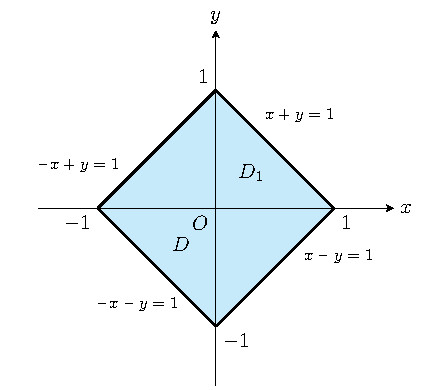
\includegraphics[width=6cm]{2022x-figure1.pdf} % 引入图片源
          \end{minipage}

    \item \textbf{Solution}.

          \noindent
          \begin{minipage}[c]{0.7\textwidth}
              积分区域如图所示.

              用极坐标代换，圆弧$y=1+\sqrt{1-x^{2}}$对应的极坐标方程为$r=2\sin \theta$，所以

              \[
                  \begin{aligned}
                      I = {} & \iint\limits_{D}xy\,\mathrm{d}x\,\mathrm{d}y = \int_{\frac{\pi}{4}}^{\frac{\pi}{2}}\,\mathrm{d}\theta\int_{0}^{2\sin \theta}r^{3}\cos \theta\sin \theta\,\mathrm{d}r                                      \\
                      = {}   & \int_{\frac{\pi}{4}}^{\frac{\pi}{2}}\cos \theta\sin \theta\,\mathrm{d}\theta\int_{0}^{2\sin \theta}r^{3}\,\mathrm{d}r = 4\int_{\frac{\pi}{4}}^{\frac{\pi}{2}}\cos \theta\sin^{5} \theta\,\mathrm{d}\theta \\
                      = {}   & 4\int_{\frac{\pi}{4}}^{\frac{\pi}{2}}\sin^{5}\theta\,\mathrm{d}\sin\theta = \left.\frac{2}{3}\sin^{6}\theta\right|_{\frac{\pi}{4}}^{\frac{\pi}{2}}                                                        \\
                      = {}   & \frac{2}{3}\left(1-\frac{1}{8}\right) = \frac{7}{12}.
                  \end{aligned}
              \]
          \end{minipage}
          \hfill %
          \begin{minipage}[c]{0.4\textwidth}
              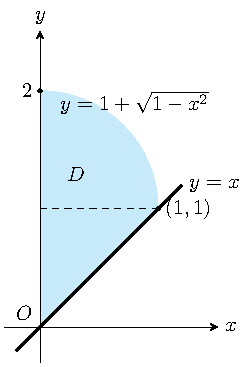
\includegraphics[width=4cm]{2022x-figure2.pdf} % 引入图片源
          \end{minipage}

    \item \textbf{Solution}. 交换积分次序，
          \[
              \begin{aligned}
                  I = {} & \int_{0}^{1}\,\mathrm{d}x\int_{x}^{1}\mathrm{e}^{-y^{2}}\,\mathrm{d}y = \int_{0}^{1}\,\mathrm{d}y\int_{0}^{y}\mathrm{e}^{-y^{2}}\,\mathrm{d}x \\
                  = {}   & \int_{0}^{1}y\mathrm{e}^{-y^{2}}\,\mathrm{d}y = -\frac{1}{2}\int_{0}^{1}\mathrm{e}^{-y^{2}}\,\mathrm{d}(-y^{2})                               \\
                  = {}   & \left.-\frac{1}{2}\mathrm{e}^{-y^{2}}\right|_{0}^{1}= \frac{1}{2}\left(1-\frac{1}{\mathrm{e}}\right).
              \end{aligned}
          \]

    \item \textbf{Solution}. 用球坐标代换，锥面$z=\sqrt{x^{2}+y^{2}}$对应的球坐标方程为$\varphi
              = \frac{\pi}{4}(z\geq 0)$，所以
          \[
              \begin{aligned}
                  I = {} & \iiint\limits_{\Omega}\frac{1}{\sqrt{x^2+y^2+z^2}}\,\mathrm{d}v = \int_{0}^{2\pi}\,\mathrm{d}\theta\int_{0}^{\frac{\pi}{4}}\,\mathrm{d}\varphi\int_{0}^{\frac{1}{\cos \varphi}}\frac{\rho^{2}\sin \varphi}{\rho}\,\mathrm{d}\rho \\
                  = {}   & 2\pi\int_{0}^{\frac{\pi}{4}}\sin \varphi\,\mathrm{d}\varphi\int_{0}^{\frac{1}{\cos \varphi}}\rho\,\mathrm{d}\rho = 2\pi\int_{0}^{\frac{\pi}{4}}\sin \varphi \cdot \frac{1}{2}\cdot \frac{1}{\cos^{2} \varphi}\,\mathrm{d}\varphi \\
                  = {}   & -\pi\int_{0}^{\frac{\pi}{4}}\frac{1}{\cos^2 \varphi}\,\mathrm{d}(\cos \varphi) = \left.\pi\cdot \frac{1}{\cos \varphi}\right|_{0}^{\frac{\pi}{4}}= \pi\left(\sqrt{2}-1\right).
              \end{aligned}
          \]
\end{enumerate}

\section{综合题(每小题 8 分，共 40 分)}
\begin{enumerate}
    \setcounter{enumi}{10}
    \item \textbf{Solution}. $\begin{cases}
                  u = x-2\sqrt{y}, \\
                  v = x+2\sqrt{y}
              \end{cases}$两边全微分，得$\begin{cases}
                  \mathrm{d}u = \mathrm{d}x - \frac{1}{\sqrt{y}}\,\mathrm{d}y, \\[6pt]
                  \mathrm{d}v = \mathrm{d}x + \frac{1}{\sqrt{y}}\,\mathrm{d}y
              \end{cases}$，

          所以$\frac{\partial u}{\partial x}= \frac{\partial v}{\partial x}= 1$，$\frac{\partial
                  u}{\partial y}= -\frac{1}{\sqrt{y}}$，$\frac{\partial v}{\partial y}= \frac{1}{\sqrt{y}}$.

          由链式法则，
          \[
              \frac{\partial z}{\partial x}= \frac{\partial z}{\partial u}\cdot
              \frac{\partial u}{\partial x}+ \frac{\partial z}{\partial v}\cdot \frac{\partial
                  v}{\partial x}= \frac{\partial z}{\partial u}+ \frac{\partial z}{\partial
                  v},
          \]
          \[
              \frac{\partial z}{\partial y}= \frac{\partial z}{\partial u}\cdot \frac{\partial
                  u}{\partial y}+ \frac{\partial z}{\partial v}\cdot \frac{\partial v}{\partial
                  y}= -\frac{1}{\sqrt{y}}\cdot \frac{\partial z}{\partial u}+ \frac{1}{\sqrt{y}}
              \cdot \frac{\partial z}{\partial v},
          \]
          \[
              \frac{\partial^{2} z}{\partial x^{2}}= \frac{\partial}{\partial x}\left(\frac{\partial
                  z}{\partial u}+ \frac{\partial z}{\partial v}\right) = \frac{\partial^{2} z}{\partial
                  u^{2}}\cdot \frac{\partial u}{\partial x}+ \frac{\partial^{2} z}{\partial
                  u\partial v}\cdot \frac{\partial v}{\partial x}+ \frac{\partial^{2} z}{\partial
                  v\partial u}\cdot \frac{\partial u}{\partial x}+ \frac{\partial^{2} z}{\partial
                  v^{2}}\cdot \frac{\partial v}{\partial x}= \frac{\partial^{2} z}{\partial
                  u^{2}}+ 2\frac{\partial^{2} z}{\partial u\partial v}+ \frac{\partial^{2} z}{\partial
                  v^{2}},
          \]
          \[
              \begin{aligned}
                  \frac{\partial^{2} z}{\partial y^{2}} = {} & \frac{\partial}{\partial y}\left(-\frac{1}{\sqrt{y}}\cdot \frac{\partial z}{\partial u} + \frac{1}{\sqrt{y}}\cdot \frac{\partial z}{\partial v}\right)                                                                                                                                                                                                                                                                                                                                                    \\
                  = {}                                       & \frac{1}{2y\sqrt{y}}\cdot \frac{\partial z}{\partial u} - \frac{1}{\sqrt{y}}\left(\frac{\partial^{2} z}{\partial u^{2}}\cdot \frac{\partial u}{\partial y} + \frac{\partial^{2} z}{\partial u \partial v}\cdot \frac{\partial v}{\partial y}\right) - \frac{1}{2y\sqrt{y}}\cdot \frac{\partial z}{\partial v} + \frac{1}{\sqrt{y}}\left(\frac{\partial^{2} z}{\partial v \partial u}\cdot \frac{\partial u}{\partial y} + \frac{\partial^{2} z}{\partial v^{2}}\cdot \frac{\partial v}{\partial y}\right) \\
                  = {}                                       & \frac{1}{2y\sqrt{y}}\cdot \left(\frac{\partial z}{\partial u} - \frac{\partial z}{\partial v}\right) + \frac{1}{y}\left(\frac{\partial^{2} z}{\partial u^{2}} - 2\frac{\partial^{2} z}{\partial u \partial v} + \frac{\partial^{2} z}{\partial v^{2}}\right).
              \end{aligned}
          \]

          所以$\frac{\partial^{2} z}{\partial x^{2}} - y\frac{\partial^{2} z}{\partial y^{2}} - \frac{1}{2}\frac{\partial z}{\partial y}=$
          \[
              \begin{aligned}
                  {}   & \left(\frac{\partial^{2} z}{\partial u^{2}} + 2\frac{\partial^{2} z}{\partial u \partial v} + \frac{\partial^{2} z}{\partial v^{2}}\right) - y\left[\frac{1}{2y\sqrt{y}}\cdot \left(\frac{\partial z}{\partial u} - \frac{\partial z}{\partial v}\right) + \frac{1}{y}\left(\frac{\partial^{2} z}{\partial u^{2}} - 2\frac{\partial^{2} z}{\partial u \partial v} + \frac{\partial^{2} z}{\partial v^{2}}\right)\right]                                                                \\
                  - {} & \frac{1}{2}\left[-\frac{1}{\sqrt{y}}\cdot \frac{\partial z}{\partial u} + \frac{1}{\sqrt{y}}\cdot \frac{\partial z}{\partial v}\right]                                                                                                                                                                                                                                                                                                                                                 \\
                  = {} & \frac{\partial^{2} z}{\partial u^{2}} + 2\frac{\partial^{2} z}{\partial u \partial v} + \frac{\partial^{2} z}{\partial v^{2}} - \frac{1}{2\sqrt{y}}\cdot \left(\frac{\partial z}{\partial u} - \frac{\partial z}{\partial v}\right) - \left(\frac{\partial^{2} z}{\partial u^{2}} - 2\frac{\partial^{2} z}{\partial u \partial v} + \frac{\partial^{2} z}{\partial v^{2}}\right) + \frac{1}{2\sqrt{y}}\cdot \left(\frac{\partial z}{\partial u} - \frac{\partial z}{\partial v}\right) \\
                  = {} & 4\frac{\partial^{2} z}{\partial u \partial v}.
              \end{aligned}
          \]

          因此$\frac{\partial^{2} z}{\partial x^{2}}- y\frac{\partial^{2} z}{\partial
                  y^{2}}- \frac{1}{2}\frac{\partial z}{\partial y}= 0 \Leftrightarrow \frac{\partial^{2}
                  z}{\partial u \partial v}= 0$.

    \item \textbf{Solution}. 当$x\to0,y\to0$时，$\frac{x^{2}y^{2}}{\left(x^{2}+y^{2}\right)^{\frac{3}{2}}}
              \leq x^{2}\sqrt{|y|}$，而$\lim_{\substack{x\to 0 \\ y\to 0}}x^{2}\sqrt{|y|}
              =0$，

          所以由夹逼定理可知$\lim_{\substack{x\to 0 \\ y\to 0}}\frac{x^{2}y^{2}}{\left(x^{2}+y^{2}\right)^{\frac{3}{2}}}
              =0=f(0,0)$，函数$f(x,y)$在原点处连续.

          又$f(x,0)=f(0,y)\equiv 0$，所以$f_{x}(0,0)=f_{y}(0,0)=0$，因此函数$f(x,y)$在原点处的偏导数存在.

          考察
          \[
              \lim_{\substack{x\to 0 \\ y\to 0}}\frac{f(x,y)-f(0,0)-f_{x}(0,0)x-f_{y}(0,0)y}{\sqrt{x^{2}+y^{2}}}
              = \lim_{\substack{x\to 0 \\ y\to 0}}\frac{x^{2} y^{2}}{\left(x^{2}+y^{2}\right)^{2}}.
          \]

          当$y=x,x\to0,y\to0$时，
          \[
              \lim_{\substack{x\to 0 \\ y\to 0}}\frac{x^{2} y^{2}}{\left(x^{2}+y^{2}\right)^{2}}
              = \lim_{x\to0}\frac{x^{4}}{(2x^{2})^{2}}= \frac{1}{4},
          \]
          所以$\lim_{\substack{x\to 0 \\ y\to 0}}
              \frac{x^{2} y^{2}}{\left(x^{2}+y^{2}\right)^{2}}\neq 0$，因此函数$f(x,y)$在原点处不可微.

    \item \textbf{Solution}. $\nabla F |_{M}= \left.\left(ay^{2}+3cx^{2} z^{2}
              , 2axy+bz, 2cx^{3} z + by\right)\right|_{(1,2,-1)}=(4a+3c, 4a-b, 2b-2c)$，

          由题意可知$\nabla F |_{M}// (1,0,0)$，所以$\begin{cases}
                  4a-b = 0,  \\
                  2b-2c = 0, \\
                  4a+3c = 64
              \end{cases}$，解得$\begin{cases}
                  a = 4,  \\
                  b = 16, \\
                  c = 16.
              \end{cases}$

    \item \textbf{Solution}.

          \noindent
          \begin{minipage}[c]{0.6\textwidth}
              由题可知旋转曲面的方程为$x^{2}+y^{2}=2z$，积分区域$\Omega$如图所示.

              用截面法，
              \[
                  \begin{aligned}
                      I = {} & \iiint\limits_{\Omega}z\,\mathrm{d}v = \int_{1}^{2}\,\mathrm{d}z\iint\limits_{x^2+y^2\leq 2z}z\,\mathrm{d}x\,\mathrm{d}y \\
                      = {}   & 2\pi\int_{1}^{2}z^{2}\,\mathrm{d}z                                                                                       \\
                      = {}   & \frac{2\pi}{3}\left(8-1\right) = \frac{14\pi}{3}.
                  \end{aligned}
              \]
          \end{minipage}
          \hfill %
          \begin{minipage}[c]{0.5\textwidth}
              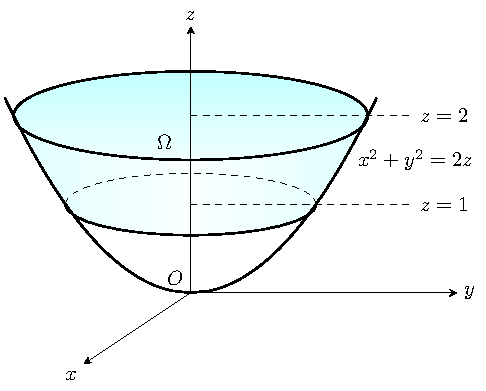
\includegraphics[width=6cm]{2022x-figure3.pdf} % 引入图片源
          \end{minipage}

    \item \textbf{Solution}. 如图所示，联立$\begin{cases}
                  x^{2}+y^{2}+z=4, \\
                  x^{2}+y^{2}+z^{2}=4z
              \end{cases}$得$4-z+z^{2}=4z$，

          解得$z=1$或$z=4$，因此抛物面和球面的交线为$x^{2}+y^{2}=3$.

          抛物面$x^{2}+y^{2}+z=4$将球体$x^{2}+y^{2}+z^{2}\leq 4z$分为$\Omega_{1}$和$\Omega
              _{2}$两部分.

          \noindent
          \begin{minipage}[c]{0.6\textwidth}
              用截面法，
              \[
                  \begin{aligned}
                      V_{2} = {} & \iiint\limits_{\Omega_2}\,\mathrm{d}v = \int_{0}^{1}\,\mathrm{d}z\iint\limits_{x^2+y^2\leq 4z-z^2}\,\mathrm{d}x\,\mathrm{d}y + \int_{1}^{4}\,\mathrm{d}z\iint\limits_{x^2+y^2\leq 4-z}\,\mathrm{d}x\,\mathrm{d}y \\
                      = {}       & \pi\int_{0}^{1}\left(4z-z^{2}\right)\,\mathrm{d}z + \pi\int_{1}^{4}\left(4-z\right)\,\mathrm{d}z                                                                                                                 \\
                      = {}       & \pi\left[\left.\left(2z^{2}-\frac{z^3}{3}\right)\right|_{0}^{1}+ \left.\left(4z-\frac{z^2}{2}\right)\right|_{1}^{4}\right]                                                                                       \\
                      = {}       & \pi\left[\left(2-\frac{1}{3}\right) + \left(16-8-4+\frac{1}{2}\right)\right]                                                                                                                                     \\
                      = {}       & \pi\left(\frac{5}{3}+ \frac{9}{2}\right) = \frac{37\pi}{6}.
                  \end{aligned}
              \]
          \end{minipage}
          \hfill %
          \begin{minipage}[c]{0.5\textwidth}
              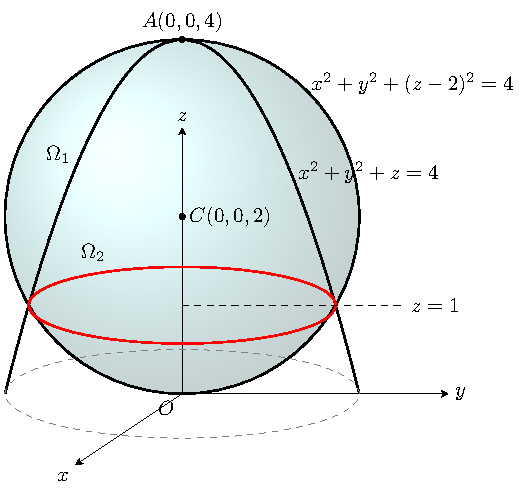
\includegraphics[width=6cm]{2022x-figure4.pdf} % 引入图片源
          \end{minipage}

          故$V_{1} = \frac{4\pi}{3}\cdot 2^{3} - V_{2} = \frac{32\pi}{3}- \frac{37\pi}{6}
              = \frac{27\pi}{6}$，所以体积比$\frac{V_{1}}{V_{2}}= \frac{27}{37}$.
\end{enumerate}
\end{document}





